% Provenance (never printed): see sources/outline_sources.md (Year 1: morphology,
% gravity, heat flow and seismicity of a subduction zone; accretionary and erosive
% margins; slab geometry; volcanic arcs). Kuril map, section and numbers from
% figdata/bachelor-1/slab_seismicity.py; exercise and problem values in the Book 3
% scratch calculator calc/ch14.py.
\chapter{Margens ativas}\label{ch:b1:active-margins}

Em 11 de março de 2011, às 14h46 pela hora local, a fronteira de placas ao largo do nordeste do Japão rompeu-se ao longo de cerca de \qty{400}{km} da fossa e \qty{150}{km} em seu \omterm{def:b1:geological-maps:attitude}{mergulho}. A falha deslizou até 50 a \qty{60}{m}, a maior parte no sentido ascendente do plano, em direção à fossa do Japão; em terra, a costa se deslocou horizontalmente e afundou. A placa que ali mergulha, a placa do Pacífico, desce sob o Japão ao longo de um plano que os terremotos delineiam até centenas de quilômetros de profundidade; e, onde esse plano está a cerca de cem quilômetros de profundidade, uma linha de vulcões corre paralela à costa. Este capítulo lê uma margem como essa a partir de sua forma, de sua gravidade, de seu \omterm{def:b1:heat-budget:heat-flow}{fluxo de calor} e, sobretudo, de seus terremotos.
% ledger: usgs:tohoku, wada:decoupling

\begin{recall}
A \omterm{def:b1:layered-earth:lithosphere}{litosfera} oceânica afunda de volta no \omterm{def:b1:layered-earth:layers}{manto} nas zonas de subducção, marcadas por fossas e por zonas inclinadas de terremotos, e a \omterm{def:b1:layered-earth:lithosphere}{litosfera} velha afunda sob o próprio peso (Livro 2, 11º ano); a água da placa que afunda reduz a temperatura de fusão do \omterm{def:b1:layered-earth:layers}{manto} acima dela (Livro 2, 12º ano). O calor se difunde por uma distância $L$ em um tempo da ordem de $L^2/\kappa$ (\cref{ch:b1:heat-budget}); uma laje infinita de densidade $\rho$ e espessura $h$ atrai com $2\pi G\rho h$ (\cref{ch:b1:isostasy-gravity}); as placas giram em torno de \omterm{def:b1:plate-kinematics:euler-pole}{polos de Euler} (\cref{ch:b1:plate-kinematics}); o \omterm{def:b1:heat-budget:heat-flow}{fluxo de calor} do fundo oceânico cai com o inverso da raiz quadrada de sua idade (\cref{ch:b1:rifts-ridges-margins}).
\end{recall}

\section{A anatomia de uma margem ativa}\label{sec:b1:active-margins:anatomy}

\begin{definition}[Margem ativa, fossa oceânica, antearco, bacia de retroarco]\label{def:b1:active-margins:active-margin}
Uma \emph{margem ativa}\index{margem ativa} é um limite convergente de placas no qual a \omterm{def:b1:layered-earth:lithosphere}{litosfera} oceânica afunda sob outra placa, seja sob um continente, seja sob outra placa oceânica. Uma \emph{fossa oceânica}\index{fossa oceânica} é a depressão longa, estreita e em forma de V do fundo do mar ao longo da qual a placa que afunda se curva para baixo sob a outra. O \emph{antearco}\index{antearco} é a parte da placa cavalgante entre a fossa e a linha de vulcões. Uma \emph{bacia de retroarco}\index{bacia de retroarco} é uma bacia atrás dos vulcões, do lado oposto à fossa, onde a placa cavalgante é estirada e pode se formar \omterm{def:b1:rifts-ridges-margins:oceanic-crust}{crosta oceânica} nova.
\end{definition}

As fossas são os lugares mais profundos dos oceanos, e o mais profundo de todos é o Challenger Deep, na fossa das Marianas. Ao longo da fossa das Curilas, o fundo desce de cerca de \qty{5200}{m} na planície abissal para \qty{8700}{m} no eixo, cerca de \qty{3.5}{km} mais baixo, e a fossa tem apenas dezenas de quilômetros de largura (figura em \cref{sec:b1:active-margins:gravity-heat}). As margens convergentes da Terra medem cerca de \qty{55000}{km} ao todo; em um modelo digital dos limites de placas, as margens de subducção somam cerca de \qty{51000}{km}, contra cerca de \qty{67000}{km} de dorsais de espalhamento.
% ledger: data:b3-grav-kuril (trench_gravity.py values), stern:subduction, data:pb2002 (ridge_budget.py)

Do lado de fora da fossa, a placa se eleva um pouco antes de mergulhar, em uma elevação externa ampla e baixa. Ali a placa está curvada, e sua parte superior está estirada: terremotos de falhas normais ocorrem nas elevações externas. A largura da elevação externa coincide com a flexão de uma placa elástica; essa flexão da \omterm{def:b1:layered-earth:lithosphere}{litosfera} é estudada no Livro 5. A própria fossa é o lugar onde o peso da placa densa que afunda puxa sua borda dianteira para baixo.

\begin{definition}[Laje em subducção]\label{def:b1:active-margins:slab}
A \emph{laje em subducção}\index{laje em subducção} é a parte da placa que afunda e que já desceu para o \omterm{def:b1:layered-earth:layers}{manto}: uma lâmina de \omterm{def:b1:layered-earth:lithosphere}{litosfera} oceânica, com a \omterm{def:b1:layered-earth:layers}{crosta} por cima, inclinada sob a placa cavalgante desde a fossa até profundidades de várias centenas de quilômetros.
\end{definition}

A placa cavalgante é cortada em faixas paralelas à fossa (figura abaixo): o \omterm{def:b1:active-margins:active-margin}{antearco}, frequentemente com uma pilha de sedimentos raspados em sua frente e uma bacia sedimentar atrás; o \omterm{def:b1:active-margins:volcanic-arc}{arco vulcânico}; e, atrás de alguns arcos, uma \omterm{def:b1:active-margins:active-margin}{bacia de retroarco} e, além dela, um arco antigo extinto. Entre a laje e a placa cavalgante fica uma cunha de \omterm{def:b1:layered-earth:layers}{manto}, arrastada para baixo ao longo do topo da laje.

\begin{omfigure}
\begin{tikzpicture}[x=0.01667cm, y=0.01667cm, font=\scriptsize,
  lbl/.style={fill=white, fill opacity=0.8, text opacity=1, inner sep=1pt}]
\begin{scope}
\clip (-150,-330) rectangle (650,55);
% mantle and sea water
\fill[orange!12] (-150,-330) rectangle (650,15);
\fill[omSea!45] (-150,15) rectangle (650,0);
% incoming plate and slab: top dips 25 deg to 50 km, then 45 deg; 100 km thick
\fill[omLithBasalt!55] (-150,4) -- (-80,4) .. controls (-60,7) and (-40,7) .. (-25,4) -- (0,0)
  -- (107.2,-50) -- (420,-363) -- (349,-434) -- (48.9,-133.1) -- (-22.1,-100) -- (-150,-100) -- cycle;
\draw[omSea!50!black, line width=1.6pt] (-150,4) -- (-80,4) .. controls (-60,7) and (-40,7) .. (-25,4) -- (0,0) -- (107.2,-50) -- (420,-363);
% overriding plate
\fill[brown!28] (0,0) -- (12,3) -- (45,8) -- (60,10) -- (140,10) -- (150,12) -- (184,12) -- (230,9)
  -- (300,7) -- (395,6) -- (410,3) -- (420,2) -- (430,3) -- (445,6) -- (540,7) -- (560,14) -- (590,14)
  -- (610,10) -- (650,10) -- (650,-60) -- (520,-55) -- (445,-25) -- (420,-15) -- (395,-25) -- (320,-55)
  -- (250,-60) -- (117.2,-60) -- (107.2,-50) -- cycle;
% accretionary prism and forearc basin
\fill[yellow!55] (0,0) -- (12,3) -- (45,8) -- (60,10) -- (60,-28) -- cycle;
\draw[black!45, line width=0.3pt] (14,-3) -- (24,5) (28,-7) -- (38,6) (42,-14) -- (52,8);
\fill[yellow!30] (68,10) -- (132,10) -- (122,4) -- (78,4) -- cycle;
% arc volcano
\fill[black!60] (150,12) -- (167,26) -- (184,12) -- cycle;
% an isotherm: a cold tongue down the slab
\draw[omDef, dashed, line width=0.6pt] (-150,-82) -- (-30,-82) -- (40,-118) -- (300,-318)
  -- (232,-200) -- (150,-112) .. controls (130,-80) and (180,-72) .. (260,-72) -- (650,-72);
% mantle wedge flow
\draw[->, black!60, line width=0.5pt] (600,-130) .. controls (450,-135) and (300,-125) .. (215,-150)
  .. controls (205,-160) and (240,-185) .. (300,-235);
% water and melt
\foreach \x/\z in {150/-93, 172/-115, 194/-137}
  \draw[->, blue!70!black, line width=0.5pt] (\x,\z) -- (\x-6,\z+28);
\draw[red!75!black, line width=0.8pt, decorate, decoration={snake, amplitude=1.2, segment length=6}] (167,-100) -- (167,12);
% earthquakes
\foreach \x/\z in {20/-12, 45/-22, 70/-34, 95/-45, 60/-40, 85/-58, 120/-70, 135/-85, 150/-104,
  165/-112, 185/-140, 205/-150, 225/-175, 248/-195, 270/-216, 290/-242, 312/-262, 330/-282, 350/-300, 365/-318}
  \fill[black] (\x,\z) circle[radius=0.9pt];
% the 100-km level beneath the arc
\draw[black!70, densely dotted] (90,-100) -- (260,-100);
\draw[black!70, densely dotted] (167,12) -- (167,-110);
\end{scope}
\draw[black!70] (-150,-330) rectangle (650,55);
\node[lbl, anchor=south] at (-85,15) {elevação externa};
\node[lbl, anchor=south] at (0,15) {fossa};
\node[lbl, anchor=west] (pr) at (75,-28) {prisma de acreção};
\draw[black!70] (pr.west) -- (38,-6);
\node[lbl, anchor=south] at (88,15) {antearco};
\node[lbl, anchor=south] at (185,27) {arco vulcânico};
\node[lbl, anchor=south] at (420,15) {bacia de retroarco};
\node[lbl, anchor=south] at (575,15) {arco remanescente};
\node[lbl, anchor=west] at (-140,-50) {litosfera oceânica};
\node[lbl, anchor=east] (sl) at (120,-262) {laje em subducção};
\draw[black!70] (sl.east) -- (205,-262);
\node[lbl, anchor=west] (wb) at (420,-265) {zona de Wadati--Benioff};
\draw[black!70] (wb.west) -- (318,-266);
\node[lbl] at (430,-170) {cunha do manto};
\node[lbl] at (575,-30) {placa cavalgante};
\node[lbl, anchor=west, text=blue!70!black] at (212,-98) {água};
\node[lbl, anchor=east] at (88,-100) {\qty{100}{km} de profundidade};
\node[lbl, anchor=west, text=omDef] at (450,-95) {uma isoterma};
\node[lbl, anchor=west] at (-140,-300) {manto};
\draw[line width=1pt] (500,-310) -- (600,-310) node[midway, above] {\qty{100}{km}};
\end{tikzpicture}
\par\smallskip{\small Uma zona de subducção em seção (esquemática: \omterm{def:b1:layered-earth:lithosphere}{litosfera} e laje desenhadas na escala da barra de escala, topografia acima do fundo do mar muito exagerado). A laje mergulha suavemente sob o \omterm{def:b1:active-margins:active-margin}{antearco} e mais abruptamente abaixo; o \omterm{def:b1:active-margins:volcanic-arc}{arco vulcânico} se ergue acima do lugar em que o topo da laje está a cerca de \qty{100}{km} de profundidade. A laje fria arrasta suas isotermas para dentro do \omterm{def:b1:layered-earth:layers}{manto} (tracejado: uma isoterma), e o \omterm{def:b1:layered-earth:layers}{manto} da cunha é arrastado para baixo ao longo dela. Pontos: terremotos, no limite de placas perto da fossa e dentro da laje, abaixo. A água liberada pela laje sobe para a cunha; o magma sobe até o arco.}
\label{fig:b1:active-margins:section}
\end{omfigure}

Pelo mesmo modelo digital, cerca de \qty{2.7}{km^2} de fundo oceânico descem pelas fronteiras de subducção a cada ano, valor próximo dos \qty{3.0}{km^2} produzidos nas dorsais (\cref{ch:b1:rifts-ridges-margins}): dentro da precisão de um modelo assim, que deixa de fora a deformação lenta das zonas largas de fronteira de placas, o fundo oceânico é destruído tão depressa quanto é produzido, e a superfície da Terra mantém seu tamanho.
% ledger: data:pb2002 (ridge_budget.py: consumed 2.74, made 3.01 km2/yr)

\section{Gravidade e fluxo de calor}\label{sec:b1:active-margins:gravity-heat}

Felix Vening Meinesz encontrou as faixas longas e estreitas de anomalias negativas de gravidade ao longo das fossas (\cref{ch:b1:isostasy-gravity}). Hoje os satélites as mapeiam em toda parte sobre o mar. Atravessando a fossa das Curilas (figura abaixo), a anomalia ar livre sobe a cerca de \qty{40}{\milli\gal} sobre a elevação externa, cai para \qty{-260}{\milli\gal} sobre a fossa e volta a ser fortemente positiva sobre o \omterm{def:b1:active-margins:active-margin}{antearco} e as ilhas do arco.
% ledger: egs:vening-meinesz, data:b3-grav-kuril (trench_gravity.py values: rise 38 mGal at -155 km, low -260 at 0, high 218 at 160 km)

O tamanho da anomalia da fossa diz como a fossa se sustenta. Suponhamos que a fossa, \qty{3.5}{km} mais funda que o fundo ao redor, não fosse compensada de modo algum: onde está a fossa, \qty{3.5}{km} de rocha de densidade cerca de \qty{2700}{kg.m^{-3}} são substituídos por água do mar. Pela laje de Bouguer (\cref{prop:b1:isostasy-gravity:slab}), a gravidade ali seria menor em
\[
  2\pi G\,\Delta\rho\,h = 2\pi \times \num{6.674e-11} \times 1700 \times 3500
  \approx \qty{2.5e-3}{m.s^{-2}} = \qty{250}{\milli\gal} .
\]
Esse é o tamanho do mínimo observado. Uma fossa, portanto, não está em equilíbrio isostático: é uma depressão mantida para baixo, pela resistência da placa curvada e pela tração da laje, contra a flutuabilidade do \omterm{def:b1:layered-earth:layers}{manto} abaixo. (Uma fossa com apenas dezenas de quilômetros de largura atrai menos que uma laje infinita, de modo que a água que ela contém, sozinha, dá um pouco menos que isso; o restante do déficit está mais fundo, onde toda a placa curvada, com sua \omterm{def:b1:layered-earth:layers}{crosta} leve, é empurrada para dentro do \omterm{def:b1:layered-earth:layers}{manto}: exercício~\ref{exo:b1:active-margins:1}.)

\begin{omfigure}
\begin{tikzpicture}
\begin{axis}[omrecord, name=grav, width=0.86\linewidth, height=4.6cm, xmin=-250, xmax=450,
  ymin=-300, ymax=260, ylabel={anomalia ar livre (\unit{\milli\gal})}, ylabel style={at={(-0.075,0.5)}}, xticklabels={},
  ytick={-200,-100,0,100,200}, clip=false]
% computed in figdata/bachelor-1/trench_gravity.py; ledger: data:b3-grav-kuril
\addplot[black!30, forget plot] coordinates {(-250,0) (450,0)};
\addplot[omDef, line width=1pt] table[x=x, y=faa] {figdata/out/bachelor-1-trench_gravity-profile.dat};
\draw[black!50, densely dotted] (axis cs:0,-300) -- (axis cs:0,260) (axis cs:164,-300) -- (axis cs:164,260);
\node[font=\scriptsize, anchor=south] at (axis cs:-155,45) {elevação externa, $+38$};
\node[font=\scriptsize, anchor=west] at (axis cs:12,-262) {fossa, $-260$};
\node[font=\scriptsize, anchor=south west] at (axis cs:200,140) {antearco e arco};
\end{axis}
\begin{axis}[omrecord, at={(grav.south)}, anchor=north, yshift=-0.45cm, width=0.86\linewidth, height=4.6cm,
  xmin=-250, xmax=450, ymin=20, ymax=100, ylabel={fluxo de calor (\unit{mW.m^{-2}})}, ylabel style={at={(-0.075,0.5)}},
  xlabel={distância da fossa, em direção à placa cavalgante (\unit{km})}, clip=false]
% schematic; levels from the ledger: parsons:plate-model (11.3/sqrt(122) x 41.84 = 42.8 mW/m2 for the
% 122-Myr Kuril plate), hyndman:backarc (70-85); the forearc low is drawn without a value (wada:decoupling)
\addplot[fill=omDef!15, draw=none, forget plot] coordinates {(190,70) (450,70) (450,85) (190,85)} -- cycle;
\addplot[omProp!80!black, line width=1pt, smooth, tension=0.5] coordinates {(-250,43) (-60,43) (-10,41) (30,36) (120,36)
  (150,48) (180,76) (230,78) (450,78)};
\draw[black!50, densely dotted] (axis cs:0,20) -- (axis cs:0,100) (axis cs:164,20) -- (axis cs:164,100);
\node[font=\scriptsize, anchor=south] at (axis cs:-130,44) {fundo oceânico antigo, cerca de 43};
\node[font=\scriptsize, anchor=north] at (axis cs:75,34) {antearco: mais baixo};
\node[font=\scriptsize, anchor=south] at (axis cs:320,85) {arco e retroarco, 70 a 85};
\node[font=\scriptsize, anchor=north west] at (axis cs:3,99) {fossa};
\node[font=\scriptsize, anchor=north west] at (axis cs:167,99) {arco};
\end{axis}
\end{tikzpicture}
\par\smallskip{\small Gravidade e \omterm{def:b1:heat-budget:heat-flow}{fluxo de calor} através de uma zona de subducção. Em cima: a anomalia de gravidade ar livre medida por satélite ao longo do corte da figura em \cref{sec:b1:active-margins:seismicity}, das Curilas: \qty{38}{\milli\gal} sobre a elevação externa, \qty{-260}{\milli\gal} sobre a fossa, fortemente positiva sobre o \omterm{def:b1:active-margins:active-margin}{antearco} e as ilhas. Embaixo: o \omterm{def:b1:heat-budget:heat-flow}{fluxo de calor}, um perfil esquemático: cerca de \qty{43}{mW.m^{-2}} sobre o fundo oceânico antigo, mais baixo sobre o \omterm{def:b1:active-margins:active-margin}{antearco}, de 70 a \qty{85}{mW.m^{-2}} em média sobre o arco e o retroarco. Pontilhado: a fossa e a frente vulcânica. Dados: modelo de gravidade marinha da Scripps Institution of Oceanography (Sandwell e outros, 2014).}
\label{fig:b1:active-margins:profiles}
\end{omfigure}

O \omterm{def:b1:heat-budget:heat-flow}{fluxo de calor} conta a mesma história pelo outro lado. O fundo oceânico velho que chega a uma fossa perde pouco calor: cerca de \qty{43}{mW.m^{-2}} pela lei de \cref{ch:b1:rifts-ridges-margins}, para a placa de Curilas, com \qty{122}{Myr}. Sobre o \omterm{def:b1:active-margins:active-margin}{antearco} o fluxo é ainda menor: a laje fria sob ele absorve calor de cima, e o \omterm{def:b1:layered-earth:layers}{manto} sob o \omterm{def:b1:active-margins:active-margin}{antearco} é frio e estagnado. Sobre o arco e o retroarco ele é alto, de 70 a \qty{85}{mW.m^{-2}} em média, o dobro do fluxo dos interiores antigos dos continentes (cerca de \qty{40}{mW.m^{-2}}). Um \omterm{def:b1:active-margins:volcanic-arc}{arco vulcânico} ativo precisa de uma cunha de \omterm{def:b1:layered-earth:layers}{manto} a cerca de \qty{1200}{\celsius} a uns \qty{100}{km} de profundidade; atrás dele, todo o retroarco é quente, com uma \omterm{def:b1:layered-earth:lithosphere}{litosfera} de apenas 50 a \qty{60}{km} de espessura e seu \omterm{def:b1:layered-earth:discontinuity}{Moho} a 800 a \qty{900}{\celsius}.
% ledger: parsons:plate-model (11.3/sqrt(122) x 41.84 = 42.8), wada:decoupling, hyndman:backarc

Por que a laje permanece fria? Ela afunda mais depressa do que consegue aquecer. A laje das Curilas de \cref{sec:b1:active-margins:seismicity} entra na fossa a cerca de \qty{82}{mm} por ano e mergulha a \ang{45}: atinge \qty{600}{km} após um percurso de $600/\sin\ang{45} \approx \qty{850}{km}$, em cerca de dez milhões de anos. Pela escala de tempo condutiva (\cref{prop:b1:heat-budget:timescale}), o calor do \omterm{def:b1:layered-earth:layers}{manto} leva para atravessar os \qty{50}{km} até o meio de uma laje de \qty{100}{km} de espessura em
\[
  \tau = \frac{L^2}{\kappa} = \frac{(\qty{5e4}{m})^2}{\qty{e-6}{m^2.s^{-1}}}
  = \qty{2.5e15}{s} \approx \qty{80}{Myr},
\]
A parte central da laje chega a \qty{600}{km} quase tão fria quanto estava na fossa, e as isotermas são arrastadas com ela, como mostra a seção de uma zona de subducção acima.
% values (slab_seismicity.py): vel_normal 81.66 mm/yr, dip 44.9; calc/ch14.py

\section{Terremotos e a forma da laje}\label{sec:b1:active-margins:seismicity}

\begin{definition}[Zona de Wadati--Benioff]\label{def:b1:active-margins:wadati-benioff}
Uma \emph{zona de Wadati--Benioff}\index{zona de Wadati--Benioff} é a zona inclinada de terremotos que começa perto de uma fossa e se aprofunda sob a placa cavalgante, até cerca de \qty{700}{km}: ela delineia a \omterm{def:b1:active-margins:slab}{laje em subducção}.
\end{definition}
% ledger: usgs:deepest

Seus terremotos são de dois tipos. Até algumas dezenas de quilômetros de profundidade, eles ocorrem na própria fronteira de placas, na falha de \omterm{def:b1:geological-maps:attitude}{mergulho} suave ao longo da qual as duas placas deslizam uma em relação à outra; os maiores terremotos da Terra, como o de 2011 ao largo do Japão, rompem essa falha. Mais fundo, ocorrem dentro da laje, que sozinha ainda está fria o bastante para armazenar tensão. Nas maiores profundidades, mesmo a laje deve fluir em vez de romper, e como começam os terremotos profundos ainda é debatido. O terremoto mais profundo do catálogo, de magnitude 4.2, ocorreu sob a região de Vanuatu em 2004, a \qty{735.8}{km}. Em toda zona de subducção examinada, a zona é dupla em profundidades intermediárias: duas camadas de terremotos, mais afastadas uma da outra nas placas mais velhas.
% ledger: usgs:deepest, brudzinski:double, usgs:tohoku

As ilhas Curilas, entre Hokkaido e Kamchatka, estão sobre uma laje que os terremotos delineiam desde a fossa até mais de \qty{600}{km}. Ali a placa do Pacífico, com cerca de 120 milhões de anos onde chega à fossa, afunda sob a placa de Okhotsk (mapa abaixo). Os terremotos de magnitude 5 ou mais desde 1976 desenham a laje em planta: rasos ao longo da fossa, intermediários sob as ilhas, profundos sob o mar de Okhotsk. Em 24 de maio de 2013, um terremoto de magnitude 8.3 ocorreu a \qty{598}{km} sob o mar de Okhotsk, na mesma laje mais ao norte; ele foi sentido até Moscou, a cerca de \qty{6400}{km} de distância.
% values (slab_seismicity.py): age_in 121.8 Myr (median of the cells 100-400 km seaward)
% ledger: data:b3-usgs-kuril, data:b2-seafloor-age, data:pb2002, usgs:okhotsk-2013

\begin{omfigure}
\begin{tikzpicture}
\begin{axis}[x=0.40cm, y=0.598cm, xmin=138, xmax=165, ymin=40, ymax=56,
  axis background/.style={fill=omSea!35}, axis on top,
  xtick={140,145,...,165}, ytick={40,45,...,55},
  xticklabel={$\pgfmathprintnumber{\tick}^\circ$L}, yticklabel={$\pgfmathprintnumber{\tick}^\circ$N},
  tick label style={font=\scriptsize}, grid=major, grid style={gray!25, line width=0.25pt},
  legend style={font=\scriptsize, at={(0.98,0.02)}, anchor=south east, cells={anchor=west}},
  clip=true]
% computed in figdata/bachelor-1/slab_seismicity.py; ledger: data:b3-usgs-kuril, data:gvp, data:pb2002
\addplot[fill=omLithAlluv, draw=black!45, line width=0.2pt, unbounded coords=jump, forget plot] table {figdata/out/bachelor-1-slab_seismicity-map-land.dat};
\addplot[only marks, mark=*, mark size=0.45pt, black!35] table {figdata/out/bachelor-1-slab_seismicity-map-qshallow.dat};
\addlegendentry{mais rasos que \qty{70}{km}}
\addplot[only marks, mark=*, mark size=0.8pt, orange!85!black] table {figdata/out/bachelor-1-slab_seismicity-map-qmid.dat};
\addlegendentry{de 70 a \qty{300}{km}}
\addplot[only marks, mark=*, mark size=1.0pt, omDef] table {figdata/out/bachelor-1-slab_seismicity-map-qdeep.dat};
\addlegendentry{mais profundos que \qty{300}{km}}
\addplot[only marks, mark=triangle*, mark size=1.6pt, black, fill=red!70!black] table {figdata/out/bachelor-1-slab_seismicity-map-volc.dat};
\addlegendentry{vulcão do Holoceno}
\addplot[black, line width=0.6pt, unbounded coords=jump, forget plot] table {figdata/out/bachelor-1-slab_seismicity-map-trench.dat};
\addplot[fill=black, draw=none, unbounded coords=jump, forget plot] table {figdata/out/bachelor-1-slab_seismicity-map-teeth.dat};
\addplot[omProp, line width=0.8pt, dashed, forget plot] table {figdata/out/bachelor-1-slab_seismicity-map-strip.dat};
\node[font=\scriptsize, fill=white, fill opacity=0.8, text opacity=1, inner sep=1pt] at (axis cs:147,54.3) {mar de Okhotsk};
\node[font=\scriptsize, fill=white, fill opacity=0.8, text opacity=1, inner sep=1pt] at (axis cs:158.5,44) {placa do Pacífico};
\node[font=\scriptsize, fill=white, fill opacity=0.8, text opacity=1, inner sep=1pt] at (axis cs:157.2,55.2) {Kamchatka};
\node[font=\scriptsize, fill=white, fill opacity=0.8, text opacity=1, inner sep=1pt] at (axis cs:139.7,44.3) {Hokkaido};
\node[font=\scriptsize, fill=white, fill opacity=0.8, text opacity=1, inner sep=1pt, rotate=40] at (axis cs:155.6,46.4) {fossa das Curilas};
\node[font=\scriptsize, fill=white, fill opacity=0.8, text opacity=1, inner sep=1pt, text=omProp] at (axis cs:146.3,51.4) {corte};
\end{axis}
\end{tikzpicture}
\par\smallskip{\small A zona de subducção das Curilas: terremotos de magnitude 5 ou mais, de 1976 a 2025, coloridos pela profundidade, e os vulcões ativos nos últimos dez mil anos. A fossa (dentes na placa cavalgante) e a faixa do corte mostrado na figura seguinte (tracejado, \qty{150}{km} de cada lado da linha de corte). Dados: catálogo de terremotos do USGS; Smithsonian Global Volcanism Program; fossa a partir de Bird (2003); costa a partir do Natural Earth.}
\label{fig:b1:active-margins:map}
\end{omfigure}

Para ver a laje em corte, mantenha os terremotos a menos de \qty{150}{km} de uma linha que parte da fossa e corre perpendicularmente a ela, em direção à placa cavalgante, e marque cada um à sua distância $x$ ao longo da linha e à sua profundidade $z$ (figura abaixo). Os pontos formam uma faixa; a reta que melhor a acompanha é encontrada pelo método dos mínimos quadrados.

\begin{method}[Ajuste da laje por mínimos quadrados]\label{met:b1:active-margins:lsq}
Dados $n$ terremotos em $(x_i, z_i)$ dentro da laje:
\begin{enumerate}
  \item calcule as médias $\bar x = \frac1n\sum x_i$ e $\bar z = \frac1n\sum z_i$;
  \item calcule $S_{xx} = \sum (x_i - \bar x)^2 = \sum x_i^2 - n\bar x^2$ e
        $S_{xz} = \sum (x_i - \bar x)(z_i - \bar z) = \sum x_i z_i - n\bar x\bar z$;
  \item a reta da laje é $z = a + s x$, com $s = S_{xz}/S_{xx}$ e
        $a = \bar z - s\bar x$; seu \omterm{def:b1:geological-maps:attitude}{mergulho} é $\delta = \arctan s$.
\end{enumerate}
\end{method}

A reta minimiza a soma dos quadrados dos desvios verticais
$F(a, s) = \sum_i (z_i - a - s x_i)^2$, uma função quadrática de $a$ e $s$ que é mínima onde as duas derivadas parciais se anulam. $\partial F/\partial a =
-2\sum (z_i - a - s x_i) = 0$ dá $\bar z = a + s\bar x$: a reta passa pelo centro dos pontos. Substituindo $a = \bar z - s\bar x$,
$\partial F/\partial s = -2\sum x_i\,[(z_i - \bar z) - s(x_i - \bar x)] = 0$;
como $\sum \bar x\,[(z_i - \bar z) - s(x_i - \bar x)] = 0$, isso é
$\sum (x_i - \bar x)[(z_i - \bar z) - s(x_i - \bar x)] = 0$, ou seja
$S_{xz} = s S_{xx}$.

Sob as ilhas Curilas centrais, a faixa tem 599 terremotos, 121 deles mais fundos que \qty{70}{km}, dentro da laje. Os mais rasos têm pouca utilidade para o ajuste: misturam a fronteira de placas e a placa em curvatura, e 147 dos 478 estão registrados na mesma profundidade redonda de \qty{33}{km}. Os 121 mais profundos dão
\[
  z = -52.7 + 0.996\,x \quad\text{(quilômetros)},
\]
um \omterm{def:b1:geological-maps:attitude}{mergulho} de \ang{44.9}, cerca de \ang{45}, até o terremoto mais profundo da faixa, a \qty{632}{km}. A reta não passa pela fossa: ela atinge a superfície \qty{53}{km} para o lado do continente em relação à fossa. A laje não é reta: ela deixa a fossa com um \omterm{def:b1:geological-maps:attitude}{mergulho} mais suave e se torna mais íngreme sob o \omterm{def:b1:active-margins:active-margin}{antearco}, como mostram os terremotos rasos acima da reta.
% values (slab_seismicity.py): n_section 599, n_fit 121, fit_a -52.721, fit_s 0.996397, dip 44.8966,
% max_depth 631.9; 147 of the 478 events of 70 km or less at 33.0 km (section part)

\begin{omfigure}
\begin{tikzpicture}
\begin{axis}[omrecord, omdepth, scale only axis, width=11.25cm, height=8.75cm,
  xmin=-100, xmax=800, ymin=0, ymax=700,
  xlabel={distância da fossa, em direção ao mar de Okhotsk (\unit{km})},
  ylabel={profundidade (\unit{km})}, clip=false,
  legend style={font=\scriptsize, at={(0.02,0.02)}, anchor=south west, cells={anchor=west}}]
% computed in figdata/bachelor-1/slab_seismicity.py; ledger: data:b3-usgs-kuril, data:gvp, data:pb2002
\addplot[only marks, mark=*, mark size=0.7pt, black!30] table[x=x, y=depth, restrict y to domain=0:70] {figdata/out/bachelor-1-slab_seismicity-section.dat};
\addlegendentry{mais rasos que \qty{70}{km}}
\addplot[only marks, mark=*, mark size=1.0pt, black!80] table[x=x, y=depth, restrict y to domain=70.01:800] {figdata/out/bachelor-1-slab_seismicity-section.dat};
\addlegendentry{mais profundos (ajustados)}
\addplot[omProp, line width=1pt, domain=60:740, samples=2] {-52.721 + 0.996397*x};
\addlegendentry{reta de mínimos quadrados, mergulho \ang{45}}
\addplot[only marks, mark=triangle*, mark size=3pt, omDef, forget plot] coordinates {(0,0)};
\addplot[only marks, mark=triangle*, mark size=3pt, red!70!black, forget plot] coordinates {(163.9,0)};
\draw[black!70, densely dashed] (axis cs:163.9,0) -- (axis cs:163.9,110.6);
\node[font=\scriptsize, anchor=north, text=omDef] at (axis cs:0,-28) {fossa};
\node[font=\scriptsize, anchor=south, text=red!70!black] at (axis cs:175,-8) {frente vulcânica};
\draw[black!70] (axis cs:166,110.6) -- (axis cs:290,80);
\node[font=\scriptsize, anchor=west, fill=white, fill opacity=0.8, text opacity=1, inner sep=1pt] at (axis cs:290,80) {laje a \qty{111}{km} abaixo da frente};
\end{axis}
\end{tikzpicture}
\par\smallskip{\small A laje das Curilas em corte, sem \omterm{def:b1:cross-sections:section}{exagero vertical}: os terremotos da faixa do mapa acima, à sua distância da fossa e à sua profundidade. A reta de mínimos quadrados pelos 121 terremotos mais profundos que \qty{70}{km} mergulha \ang{45}. O primeiro vulcão da faixa, a \qty{164}{km} da fossa, se ergue acima do lugar em que a reta está a \qty{111}{km} de profundidade. Dados: catálogo de terremotos do USGS; Smithsonian Global Volcanism Program; fossa a partir de Bird (2003).}
\label{fig:b1:active-margins:kuril-section}
\end{omfigure}

Uma laje fria é mais densa que o \omterm{def:b1:layered-earth:layers}{manto} ao redor, e seu peso puxa a placa atrás dela: esta é a tração da laje vista no Livro 2, 11º ano. Seu tamanho decorre da profundidade do fundo oceânico.

\begin{proposition}[O peso em excesso de uma laje]\label{prop:b1:active-margins:slab-weight}
Sob as hipóteses da \omterm{thm:b1:rifts-ridges-margins:depth-age}{lei profundidade--idade}
(\cref{thm:b1:rifts-ridges-margins:depth-age}), uma placa de idade $A$ carrega, por unidade de área, o excesso de massa
\[
  m = (\rho_m - \rho_w)\bigl(d(A) - d_r\bigr)
    = \frac{2}{\sqrt\pi}\,\rho_m\,\alpha\,(T_m - T_0)\sqrt{\kappa A}
\]
sobre o \omterm{def:b1:layered-earth:layers}{manto} a $T_m$. Uma laje dessa placa, de comprimento $L$ ao longo de seu \omterm{def:b1:geological-maps:attitude}{mergulho}
$\delta$ e ainda não aquecida, tem o peso em excesso $F = g\,m\,L$ por unidade de comprimento de fossa, do qual $F\sin\delta$ atua ao longo da laje.
\end{proposition}

\begin{proof}
Uma camada $\mathrm dz$ da placa à temperatura $T$ tem a massa $\rho_m\bigl(1 + \alpha(T_m - T)\bigr)\mathrm dz$ por unidade de área, isto é, $\rho_m\alpha(T_m - T)\,\mathrm dz$ a mais que o \omterm{def:b1:layered-earth:layers}{manto} a $T_m$. Somado sobre a placa, esse excesso vale $\rho_m\alpha\int_0^\infty (T_m - T)\,\mathrm dz$, que a demonstração da \omterm{thm:b1:rifts-ridges-margins:depth-age}{lei profundidade--idade} mostrou ser igual tanto a $(\rho_m - \rho_w)(d - d_r)$ quanto a $(2/\sqrt\pi)\rho_m\alpha(T_m - T_0)
\sqrt{\kappa A}$. Uma laje de comprimento $L$ tem, por unidade de comprimento de fossa, a área $L$ e portanto o excesso de massa $mL$, cujo peso é vertical; sua componente ao longo de uma reta que mergulha de $\delta$ é $F\sin\delta$.
\end{proof}

O fundo oceânico assim pesa o seu próprio excesso de massa: cada metro que ele afundou abaixo da dorsal corresponde a \qty{2300}{kg} de excesso por metro quadrado. Para a placa de Curilas, com \qty{122}{Myr}, a lei do semiespaço ($C = 393$), que para um fundo tão velho superestima um pouco o afundamento (\cref{ch:b1:rifts-ridges-margins}), dá $d - d_r = 393\sqrt{122} = \qty{4340}{m}$ e $m = 2300\times4340 \approx \qty{1.0e7}{kg.m^{-2}}$, dez mil toneladas em cada metro quadrado.
Até o terremoto mais profundo, a \qty{632}{km}, a laje tem $632/\sin\ang{45} = \qty{894}{km}$ de comprimento, logo
\[
  F = 9.81 \times \num{1.0e7} \times \num{8.94e5} \approx \qty{8.8e13}{N}
  \text{ por metro de fossa},
\]
dos quais \qty{6.2e13}{N.m^{-1}} ao longo da laje. Esta é uma cota superior: a laje aquece em suas faces, e grande parte de seu peso é sustentada pelo \omterm{def:b1:layered-earth:layers}{manto} viscoso que ela empurra para o lado, em vez de ser transmitido à placa na superfície. Mesmo assim, desde as análises das forças motoras de todas as placas, feitas nos anos 1970, acredita-se que a densidade em excesso da \omterm{def:b1:layered-earth:lithosphere}{litosfera} que afunda forneça a maior parte da energia que move as placas.
% ledger: forsyth:forces, stern:subduction, parsons:plate-model; values: calc/ch14.py (2300 x 393 x sqrt(122) = 9.98e6 kg/m2;
% L = 893.8 km; F = 8.75e13 N/m, along dip 6.19e13 N/m)

\section{Margens acrescionárias e erosivas}\label{sec:b1:active-margins:prisms}

A placa que afunda leva seus sedimentos até a fossa. Alguns são raspados e ficam; outros descem com a laje, e a laje pode até levar consigo rocha da placa cavalgante.

\begin{definition}[Prisma de acreção, erosão tectônica]\label{def:b1:active-margins:accretionary}
Um \emph{prisma de acreção}\index{prisma de acreção} é uma cunha de sedimentos, com fatias de \omterm{def:b1:rifts-ridges-margins:oceanic-crust}{crosta oceânica}, raspada da placa que afunda e acrescentada à frente da placa cavalgante em uma fossa. A \emph{erosão tectônica}\index{erosão tectônica} é a remoção de rocha da placa cavalgante pela placa que afunda, que a leva para baixo: a partir da frente da placa cavalgante, ou da base de sua \omterm{def:b1:layered-earth:layers}{crosta}.
\end{definition}

Um prisma cresce de duas maneiras. Na sua frente, os sedimentos são empurrados da placa que afunda e empilhados em fatias que mergulham afastando-se da fossa; as fatias mais jovens são as mais externas, e as mais antigas, mais atrás, são erguidas e tornadas mais íngremes. Na sua base, sedimentos levados para baixo ao longo da fronteira de placas ficam colados sob ele, um crescimento chamado subplaqueamento. As rochas do complexo Franciscano, na Califórnia, são um prisma antigo cujas partes subplaqueadas são hoje misturas caóticas de blocos em uma matriz cisalhada, as mélanges. Um prisma, como um monte de areia empurrado por um trator de lâmina, mantém uma inclinação constante: depois que o ângulo entre sua superfície e sua base atinge um valor crítico, ele cresce apenas como uma cópia maior de si mesmo (exercício~\ref{exo:b1:active-margins:11}).

Se uma margem constrói um prisma ou perde rocha depende do sedimento que chega à fossa e da velocidade de convergência. Margens acrescionárias, como Cascádia, as Aleutas e o sul da fossa Peru--Chile, recebem muito. Margens erosivas, como o norte da fossa Peru--Chile, Tonga--Kermadec ou as Marianas, recebem pouco, e a placa que afunda rói sua frente e a base de sua \omterm{def:b1:layered-earth:layers}{crosta}. A erosão predomina onde as placas convergem mais depressa que cerca de \qty{6}{cm} por ano e a cobertura de sedimentos tem menos de \qty{1}{km} de espessura; a acreção, onde a convergência é mais lenta ou os sedimentos da fossa têm mais de \qty{1}{km} de espessura.
% ledger: clift:erosion

\section{Arcos vulcânicos e bacias de retroarco}\label{sec:b1:active-margins:arcs}

\begin{definition}[Arco vulcânico, lacuna arco--fossa]\label{def:b1:active-margins:volcanic-arc}
Um \emph{arco vulcânico}\index{arco vulcânico} é uma faixa de vulcões sobre a placa cavalgante de uma zona de subducção, paralela à fossa e convexa em direção à placa que afunda, alimentada por magma da cunha de \omterm{def:b1:layered-earth:layers}{manto} acima da laje. A \emph{lacuna arco--fossa}\index{lacuna arco--fossa} é a distância horizontal entre a fossa e a frente vulcânica, a linha de vulcões mais próxima da fossa.
\end{definition}

Os \omterm{def:b1:active-margins:volcanic-arc}{arcos vulcânicos} se erguem onde o topo da laje está, em média, a cerca de \qty{105}{km} de profundidade, embora a profundidade sob diferentes arcos, média em trechos de \qty{500}{km} de extensão, varie de 72 a \qty{173}{km}. O magma se forma onde a água liberada pela laje, à medida que seus \omterm{def:b1:rock-forming-minerals:mineral}{minerais} hidratados se decompõem, reduz a temperatura de fusão do \omterm{def:b1:layered-earth:layers}{manto} quente da cunha (Livro 2, 12º ano; os magmas dos arcos são estudados no Livro 4). Sob as Curilas centrais, a frente vulcânica fica a \qty{164}{km} da fossa, onde a linha da laje das Curilas está a \qty{111}{km} de profundidade.
% ledger: syracuse:arc-depth
% values (slab_seismicity.py): x_front 163.9, slab_depth_front 110.586

\begin{proposition}[A lacuna arco--fossa]\label{prop:b1:active-margins:gap}
Suponha que o topo da laje mergulhe com $\delta_1$ desde a fossa até a profundidade $z_1$, depois com $\delta_2$ abaixo, e que a frente vulcânica esteja acima do lugar em que o topo da laje está na profundidade $H > z_1$. Então a \omterm{def:b1:active-margins:volcanic-arc}{lacuna arco--fossa} é
\[
  g = \frac{z_1}{\tan\delta_1} + \frac{H - z_1}{\tan\delta_2} .
\]
Para uma laje de \omterm{def:b1:geological-maps:attitude}{mergulho} uniforme $\delta$, $g = H/\tan\delta$. Para $z_1$, $H$ e $\delta_1$ dados, quanto mais suave o \omterm{def:b1:geological-maps:attitude}{mergulho} $\delta_2$, mais larga a lacuna.
\end{proposition}

\begin{proof}
No primeiro trecho, a laje afunda $z_1$ enquanto avança horizontalmente
$z_1/\tan\delta_1$, pois a tangente do \omterm{def:b1:geological-maps:attitude}{mergulho} é a profundidade ganha por unidade de distância horizontal. No segundo, ela afunda mais $H - z_1$ ao longo de
$(H - z_1)/\tan\delta_2$. A frente está acima do fim do segundo trecho, na soma das duas distâncias horizontais até a fossa. Com $\delta_1 = \delta_2
= \delta$, a soma é $H/\tan\delta$. Por fim, $\tan\delta_2$ cresce com $\delta_2$ em $(0, \ang{90})$, logo o segundo termo, e $g$, diminuem à medida que a laje se torna mais íngreme.
\end{proof}

Uma laje de \ang{45} com os vulcões a \qty{111}{km} acima dela colocaria a frente a \qty{111}{km} da fossa se fosse reta; a frente das Curilas está a \qty{164}{km} porque a laje mergulha mais suavemente sob o \omterm{def:b1:active-margins:active-margin}{antearco} (exercício~\ref{exo:b1:active-margins:6}).

Arcos são curvos, e sua curvatura decorre da esfera. Uma placa que desce ao \omterm{def:b1:layered-earth:layers}{manto} deve se dobrar sem se estirar, pois uma placa de dezenas de quilômetros de espessura não pode ser estirada em dezenas por cento. Sobre uma esfera, isso fixa a forma que uma placa dobrada pode ter.

\begin{proposition}[Uma casca esférica dobrada]\label{prop:b1:active-margins:shell}
Reflita a calota de uma esfera recortada por um pequeno círculo de raio angular $\rho$, no plano desse círculo. A calota refletida tem a mesma forma e o mesmo tamanho da original, de modo que a superfície é dobrada sem ser estirada; e ao longo do círculo ela é dobrada pelo ângulo $\theta = 2\rho$. Uma placa que afunda com \omterm{def:b1:geological-maps:attitude}{mergulho} $\theta$ ao longo de tal \omterm{def:b1:geological-maps:fold}{dobra} pode fazê-lo sem se estirar ao longo de um pequeno círculo de raio angular $\theta/2$.
\end{proposition}

\begin{proof}
Uma reflexão é uma isometria: a calota refletida tem os mesmos comprimentos e ângulos que a calota, e encontra a esfera exatamente ao longo do círculo, que a reflexão deixa no lugar. Sejam $O$ o centro da esfera e $P$ o centro da calota, sobre a esfera; o plano do círculo é perpendicular a $OP$. Em um ponto $M$ do círculo, o ângulo $\widehat{MOP}$ é $\rho$; o plano tangente da esfera em $M$ é perpendicular a $OM$, logo faz com o plano do círculo o ângulo $\rho$, plano que é perpendicular a $OP$. Ao cruzar o círculo em direção a $P$, a esfera portanto sobe acima do plano do círculo com o ângulo $\rho$; a calota refletida, sua imagem especular, desce abaixo desse plano com o ângulo $\rho$. Onde a esfera não dobrada prosseguiria a $\rho$ acima do plano, a superfície dobrada prossegue a $\rho$ abaixo dele: ela é dobrada pelo ângulo $\rho + \rho = 2\rho$.
\end{proof}

\begin{omfigure}
\begin{tikzpicture}[font=\scriptsize, line cap=round]
\def\R{3}\def\rh{40}
\pgfmathsetmacro{\h}{\R*cos(\rh)}
\pgfmathsetmacro{\mx}{\R*sin(\rh)}
% unbent sphere outside the cap
\draw[line width=1.1pt, omSea!60!black] ({90+\rh}:\R) arc[start angle=90+\rh, end angle=215, radius=\R];
\draw[line width=1.1pt, omSea!60!black] (-35:\R) arc[start angle=-35, end angle=90-\rh, radius=\R];
% original cap, dashed
\draw[dashed, black!50] ({90-\rh}:\R) arc[start angle=90-\rh, end angle=90+\rh, radius=\R];
% reflected cap
\draw[line width=1.1pt, omDef, domain=90-\rh:90+\rh, samples=40, variable=\t] plot ({\R*cos(\t)}, {2*\h-\R*sin(\t)});
% plane of the circle
\draw[black!60, densely dotted] (-\R-0.3,\h) -- (\R+0.3,\h);
% centre, radii
\fill (0,0) circle[radius=1pt] node[below left] {$O$};
\draw[black!60] (0,0) -- (0,\R) node[above] {$P$};
\draw[black!60] (0,0) -- (\mx,\h);
\draw[black!70] (0,0.75) arc[start angle=90, end angle=90-\rh, radius=0.75];
\node at ($(0,0)+({90-\rh/2}:0.98)$) {$\rho$};
\fill (\mx,\h) circle[radius=1pt];
\node[anchor=west] at (\mx+0.05,\h+0.1) {$M$};
% tangent directions at M: sphere continuing into the cap (rises at rho), reflected cap (goes down at rho)
\draw[black!70, ->] (\mx,\h) -- ++({180-\rh}:1.05);
\draw[omDef, ->] (\mx,\h) -- ++({180+\rh}:1.05);
\draw[black!70] ($(\mx,\h)+({180-\rh}:0.62)$) arc[start angle=180-\rh, end angle=180+\rh, radius=0.62];
\node[anchor=east, fill=white, inner sep=1pt] at ($(\mx,\h)+(180:0.64)$) {$2\rho$};
\node[anchor=north, text=omDef, fill=white, inner sep=1pt] at (0,{2*\h-\R-0.06}) {calota refletida};
\node[anchor=south east, black!60] (oc) at (-1.5,{\R+0.2}) {calota original};
\draw[black!50] (oc.east) -- ({110}:\R);
\node[anchor=west, black!60] at (\R+0.3,\h) {plano do círculo};
\node[anchor=west, omSea!60!black] at (-35:\R) {esfera não dobrada};
\end{tikzpicture}
\par\smallskip{\small Uma esfera cortada por seu centro $O$ e pelo centro $P$ de uma calota de raio angular $\rho$ (aqui \ang{40}, para tornar os ângulos visíveis). Refletida no plano de seu círculo, a calota conserva forma e tamanho; em $M$ a superfície, que continuava subindo a $\rho$ acima desse plano, agora desce a $\rho$ abaixo dele: ela é dobrada de $2\rho$.}
\label{fig:b1:active-margins:shell}
\end{omfigure}

A laje das Curilas mergulha \ang{45}, de modo que a proposição prevê um arco de raio angular de cerca de \ang{22.5}. As posições PB2002 da fossa das Curilas, de Hokkaido ao sul de Kamchatka, são melhor ajustadas por um pequeno círculo de raio \ang{21.9}, centrado perto de \ang{58.9}\,N, \ang{123.8}\,L, no leste da Sibéria, do lado da placa cavalgante. A concordância é próxima aqui, mas o modelo é grosseiro: só a parte central da mesma fossa dá \ang{18.1}. A ideia é de Charles Frank, em 1968: os arcos das Curilas--Kamchatka, das Aleutas e de Sumatra--Java, acima de lajes com \omterm{def:b1:geological-maps:attitude}{mergulho} de cerca de \ang{45}, têm todos raios de cerca de \ang{20}, ou cerca de \ang{22} medidos até suas fossas.
% values (slab_seismicity.py): arc_radius 21.8984, arc_pole 58.8803 N 123.75 E, arc_radius_central 18.1255,
% dip 44.8966; ledger: frank:arcs, data:pb2002

\begin{omfigure}
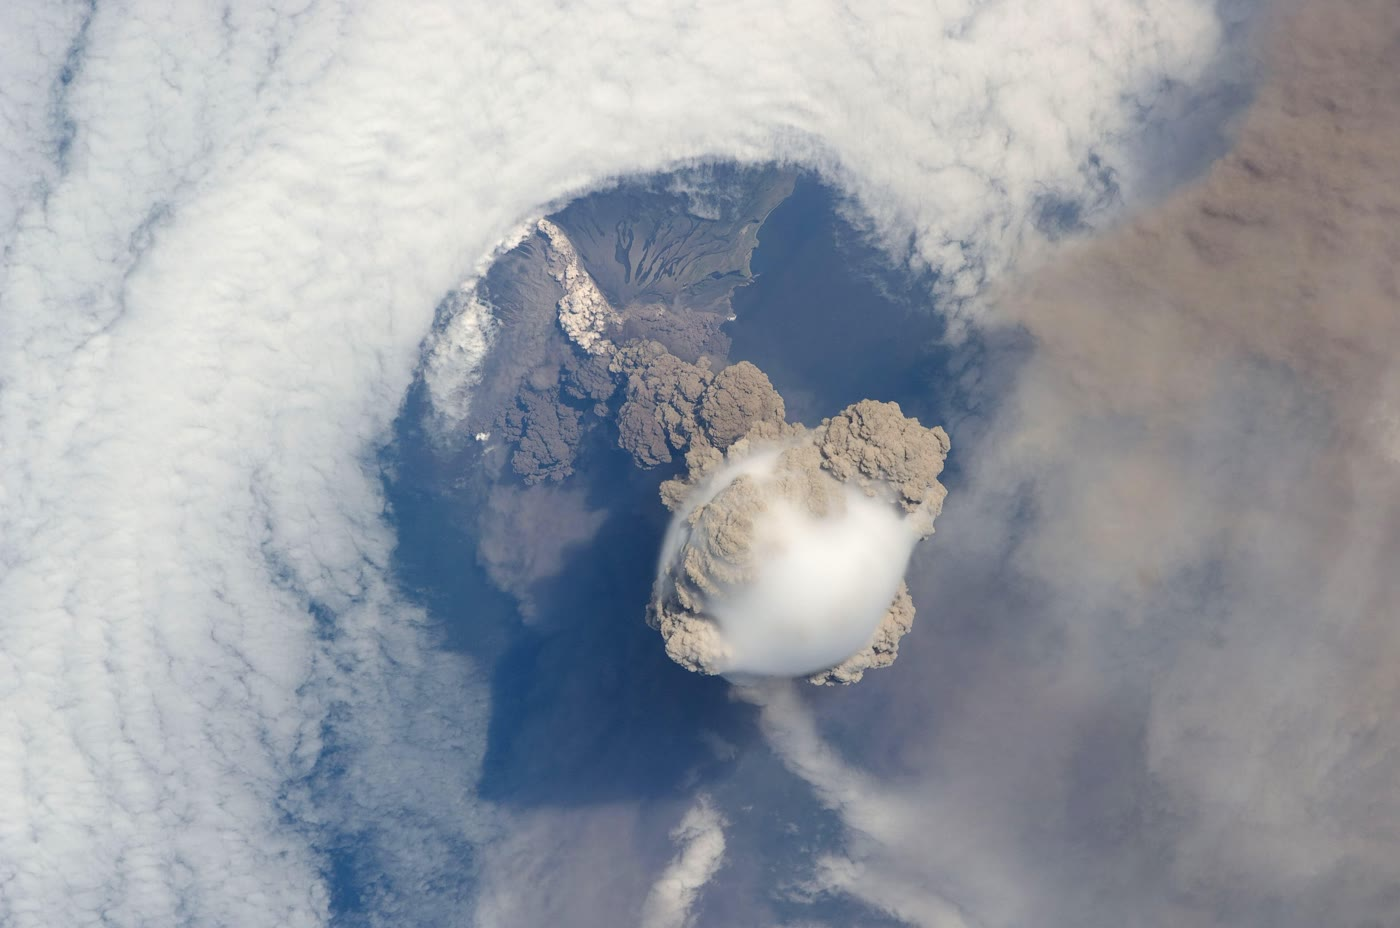
\includegraphics[width=0.66\linewidth]{images/book3/b1-sarychev-iss.jpg}
\par\smallskip{\small Sarychev Peak, um vulcão do arco das Curilas na ilha Matua, em uma fase inicial de erupção em 12 de junho de 2009, visto da Estação Espacial Internacional por uma abertura nas nuvens. Cinza acinzentada, provavelmente um fluxo piroclástico, desce do cume, e uma calota lisa de nuvem, um pileus, repousa sobre a coluna ascendente; a cinza da erupção foi detectada a mais de \qty{2400}{km} de distância. Fotografia: NASA, domínio público (Wikimedia Commons).}
\label{fig:b1:active-margins:sarychev}
\end{omfigure}
% ledger: nasa:sarychev, commons:sarychev

A \omterm{def:b1:layered-earth:layers}{crosta} sob os arcos se espessa tanto por encurtamento quanto pelo magma acrescentado por baixo; sob os arcos construídos sobre continentes, como os Andes, ela está entre as mais espessas da Terra.

Atrás de alguns arcos, a placa cavalgante é separada. Dan Karig explicou essas bacias marginais do Pacífico ocidental dentro da tectônica de placas, em 1971: quando a laje afunda de modo íngreme e recua, a fossa e o arco migram em direção à placa que afunda, e a placa atrás deles é estirada até se romper, deixando às vezes um arco remanescente extinto do outro lado. No modelo de placas usado acima, o espalhamento do retroarco ocorre a cerca de \qty{32}{mm.yr^{-1}} na Calha das Marianas, perto de \ang{18}\,N, e a mais de \qty{110}{mm.yr^{-1}} no norte da Bacia de Lau, atrás de Tonga. Onde a laje é rasa, ao contrário, ela arrasta a placa cavalgante, cuja \omterm{def:b1:layered-earth:layers}{crosta} é encurtada e espessada atrás do arco, como atrás dos Andes.
% ledger: karig:marginal-basins, data:pb2002 (ridge_budget.py: Mariana 32.4, Lau 117.5 mm/yr)

\begin{inthefield}[Alerta de tsunami]
Um centro de alerta de tsunami dispõe de minutos. Em 2011, o primeiro alerta para a costa do nordeste do Japão veio cerca de três minutos depois do terremoto, a partir de uma magnitude baseada nas ondas sísmicas de curto período; para terremotos de magnitude 8 ou mais, essa magnitude é subestimada, e por isso também foi subestimada a altura do tsunami. A magnitude de momento, que não satura, levou cerca de quinze minutos: os sismógrafos de banda larga do Japão tinham sido levados além de sua faixa. Desde 2013, quando o tamanho de um terremoto tão grande é incerto, o primeiro alerta supõe o maior terremoto possível ali e descreve o tsunami em palavras, como ``enorme'', em vez de com um número; e as previsões se apoiam em medições no mar, feitas ao largo, a partir de boias posicionadas por satélite e de medidores de pressão no fundo do mar, que veem a onda antes que ela chegue à costa.
% ledger: jma:warning

\smallskip
\begin{center}
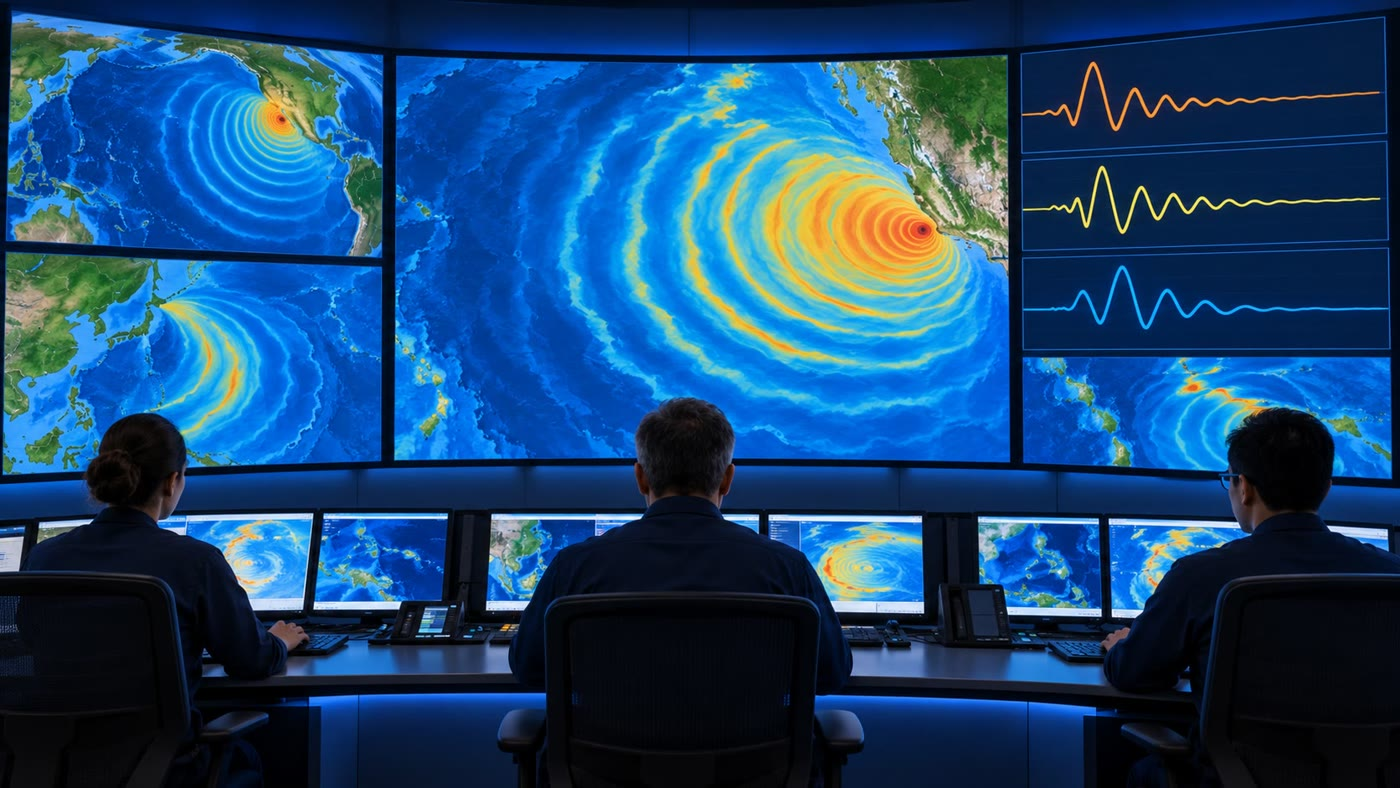
\includegraphics[width=0.7\linewidth]{images/book3/ai/b1-tsunami-centre.jpg}

{\scriptsize Plantonistas de um centro de alerta de tsunami, diante de telas com frentes de onda calculadas e registros do nível do mar (ilustração gerada por IA).}
\end{center}
\end{inthefield}

\section{Exercícios}

\begin{exercise}[$\star$]\label{exo:b1:active-margins:1}
Uma fossa fica \qty{3}{km} abaixo do fundo oceânico ao redor. (a) Se ela não fosse compensada, de quanto diminuiria a gravidade ali, pela rocha que falta, de densidade \qty{2700}{kg.m^{-3}}, substituída por água do mar de densidade \qty{1000}{kg.m^{-3}}? Use a laje de Bouguer, com $G = \qty{6.674e-11}{m^3.kg^{-1}.s^{-2}}$. (b) Compare com a anomalia observada sobre a fossa das Curilas, cerca de \qty{-260}{\milli\gal}, onde a fossa fica \qty{3.5}{km} abaixo do fundo ao redor: refaça o cálculo para essa profundidade. (c) Por que a água de uma fossa com apenas dezenas de quilômetros de largura dá menos que a fórmula da laje, e onde deve estar o restante do déficit?
\end{exercise}

\begin{exercise}[$\star$]\label{exo:b1:active-margins:2}
A placa do Pacífico entra na fossa das Curilas a \qty{82}{mm.yr^{-1}}. (a) Qual comprimento de placa desce em 10 milhões de anos? (b) Se a laje afundasse ao longo de um caminho reto com \omterm{def:b1:geological-maps:attitude}{mergulho} de \ang{45}, a que profundidade estaria então sua borda dianteira? (c) Quanto tempo leva para atingir \qty{600}{km}?
\end{exercise}

\begin{exercise}[$\star$]\label{exo:b1:active-margins:3}
Os vulcões se erguem acima do lugar em que uma laje reta está a \qty{110}{km} de profundidade. Calcule a \omterm{def:b1:active-margins:volcanic-arc}{lacuna arco--fossa} para uma laje com \omterm{def:b1:geological-maps:attitude}{mergulho} de \ang{30}, \ang{45} e \ang{60}. Qual arco fica mais distante de sua fossa?
\end{exercise}

\begin{exercise}[$\star$]\label{exo:b1:active-margins:4}
No modelo digital de placas do capítulo, cerca de \qty{2.7}{km^2} de fundo oceânico descem pelas fronteiras de subducção a cada ano, ao longo de cerca de \qty{51000}{km}, e cerca de \qty{3.0}{km^2} são produzidos ao longo de cerca de \qty{67000}{km} de dorsais de espalhamento. (a) Calcule a taxa média de convergência e a taxa média de espalhamento total, em \unit{mm.yr^{-1}}. (b) Em todas as suas fronteiras, o modelo destrói tanta área quanto produz. Para onde vai o restante do novo fundo?
% ledger: data:pb2002 (ridge_budget.py: 2.739 km2 over 51471 km; 3.009 km2 over 67340 km; all 3.511 vs 3.519)
\end{exercise}

\begin{exercise}[$\star\star$]\label{exo:b1:active-margins:5}
Quatro terremotos de um corte estão em $(x, z) = (200, 150)$, $(300, 250)$, $(400, 330)$ e $(500, 430)$, em quilômetros. (a) Ajuste a reta da laje por mínimos quadrados e dê seu \omterm{def:b1:geological-maps:attitude}{mergulho}. (b) Onde a reta atinge a superfície? (c) Compare com o \omterm{def:b1:geological-maps:attitude}{mergulho} da reta que passa apenas pelo primeiro e pelo último terremoto.
\end{exercise}

\begin{exercise}[$\star\star$]\label{exo:b1:active-margins:6}
Um modelo de laje mergulha \ang{25} desde a fossa até \qty{50}{km}, depois \ang{45}. A frente vulcânica fica onde a laje está a \qty{110}{km} de profundidade. (a) Calcule a \omterm{def:b1:active-margins:volcanic-arc}{lacuna arco--fossa}. (b) Compare com uma laje que mergulha \ang{45} o tempo todo. (c) O segmento profundo, prolongado para cima, atinge a superfície: onde? Compare com a linha das Curilas, que a atinge \qty{53}{km} para o lado do continente em relação à fossa. (d) Que lacuna daria um segmento profundo de \ang{60}?
\end{exercise}

\begin{exercise}[$\star\star$]\label{exo:b1:active-margins:7}
(a) Pela proposição da casca dobrada, qual raio angular, e qual raio em quilômetros ($R = \qty{6371}{km}$), deve ter um arco acima de uma laje com \omterm{def:b1:geological-maps:attitude}{mergulho} de \ang{45}? \ang{30}? \ang{70}? (b) Quais arcos são os mais fortemente curvados? (c) A laje das Curilas mergulha \ang{44.9} e a fossa das Curilas se ajusta a um círculo de \ang{21.9}: calcule a diferença relativa em relação à previsão.
\end{exercise}

\begin{exercise}[$\star\star$]\label{exo:b1:active-margins:8}
Considere uma condutividade de \qty{2.5}{W.m^{-1}.K^{-1}} e uma temperatura de superfície de \qty{10}{\celsius}. (a) Calcule o gradiente de temperatura sob um \omterm{def:b1:active-margins:active-margin}{antearco} que perde \qty{35}{mW.m^{-2}} e sob um retroarco que perde \qty{80}{mW.m^{-2}}. (b) Extrapolando linearmente esses gradientes, estime a temperatura a \qty{30}{km} em cada caso. (c) Os \omterm{def:b1:layered-earth:discontinuity}{Moho} de retroarco são medidos a 800 a \qty{900}{\celsius}. Por que a estimativa linear é alta demais?
% ledger: hyndman:backarc (back-arc 70-85, Moho 800-900); the forearc value is an exercise value
\end{exercise}

\begin{exercise}[$\star\star$]\label{exo:b1:active-margins:9}
No modelo de placas do capítulo, a Calha das Marianas se abre perto de \ang{18}\,N a uma taxa total de cerca de \qty{32}{mm.yr^{-1}}. (a) Exprima essa taxa em \unit{km.Myr^{-1}}, e dê a meia-taxa se o espalhamento for simétrico. (b) Quanto tempo a calha levaria para se abrir \qty{100}{km} a essa taxa? (c) Dê duas razões pelas quais a idade de uma \omterm{def:b1:active-margins:active-margin}{bacia de retroarco} não pode ser simplesmente lida de sua largura e de sua taxa atual.
% ledger: data:pb2002 (ridge_budget.py: mariana_18n_mm_yr 32.4)
\end{exercise}

\begin{exercise}[$\star\star\star$]\label{exo:b1:active-margins:10}
Uma laje com \qty{100}{km} de espessura afunda a \qty{82}{mm.yr^{-1}} ao longo de um caminho com \omterm{def:b1:geological-maps:attitude}{mergulho} de \ang{45}. Considere $\kappa = \qty{e-6}{m^2.s^{-1}}$. (a) Quanto tempo leva para atingir \qty{600}{km}? (b) Até que distância o calor se difunde para dentro dela nesse tempo, dado por $\sqrt{\kappa t}$? (c) Quanto tempo levaria o calor para chegar ao seu meio? (d) Conclua sobre a temperatura da laje a \qty{600}{km} e sobre seus terremotos.
\end{exercise}

\begin{exercise}[$\star\star\star$]\label{exo:b1:active-margins:11}
Um \omterm{def:b1:active-margins:accretionary}{prisma de acreção} modelo tem seção triangular: sua superfície se inclina de $\alpha = \ang{4}$ em direção à fossa, e sua base mergulha de $\beta = \ang{6}$ por baixo dele, ambas se encontrando em sua ponta; ele mantém esses ângulos ao crescer. (a) Mostre que sua área é $A = \frac12 L^2(\tan\alpha + \tan\beta)$ para uma largura $L$, quando os ângulos são pequenos o bastante para que a altura na parte de trás seja $L(\tan\alpha + \tan\beta)$. (b) Sedimento de \qty{1}{km} de espessura chega a uma placa que converge a \qty{40}{mm.yr^{-1}}, e todo ele é acrescido: calcule a largura após 1, 4 e 10 milhões de anos. Como $L$ cresce com o tempo? (c) E se metade do sedimento descer com a laje?
\end{exercise}

\begin{exercise}[$\star\star\star$]\label{exo:b1:active-margins:12}
(a) Mostre que a reta de mínimos quadrados passa pelo ponto médio
$(\bar x, \bar z)$. (b) Um catálogo lista cada profundidade \qty{10}{km} profunda demais. Como mudam a inclinação e a interseção da reta ajustada? (c) As distâncias $x$ são todas medidas a partir de um ponto da fossa colocado \qty{20}{km} longe demais para o lado do continente, de modo que cada $x$ é \qty{20}{km} pequeno demais. Como mudam a inclinação e a interseção? (d) Algum dos dois erros altera o \omterm{def:b1:geological-maps:attitude}{mergulho}?
\end{exercise}

\section{Problema: lendo uma zona de subducção a partir de seus terremotos}

\begin{problem}[{Problema de fim de semana --- a laje das Curilas a partir de oito terremotos, a rapidez com que ela desce, o que dizem sua gravidade e seu fluxo de calor, e onde seus vulcões devem estar}]
\label{pb:b1:active-margins:1}
% values: calc/ch14.py; the eight events are real (USGS catalogue, rounded to the km)
% from figdata/out/bachelor-1-slab_seismicity-section.dat
% ledger: data:b3-usgs-kuril, data:pb2002, data:b2-seafloor-age, syracuse:arc-depth, frank:arcs,
% data:b3-grav-kuril, parsons:plate-model, hyndman:backarc; the forearc heat flow is an exercise value
Oito terremotos da laje das Curilas, todos mais profundos que \qty{70}{km}, são listados por sua distância $x$ da fossa ao longo da linha de corte, em direção ao mar de Okhotsk, e por sua profundidade $z$, ambas arredondadas ao quilômetro.

\begin{center}
\small
\begin{tabular}{lcccccccc}
\hline
evento & 1 & 2 & 3 & 4 & 5 & 6 & 7 & 8\\
$x$ (\unit{km}) & 155 & 222 & 305 & 319 & 431 & 533 & 578 & 609\\
$z$ (\unit{km}) & 96 & 169 & 245 & 272 & 389 & 489 & 518 & 573\\
magnitude & 5.5 & 5.1 & 5.0 & 5.4 & 5.3 & 5.3 & 5.2 & 6.4\\
\hline
\end{tabular}
\end{center}

\medskip
\noindent\textbf{Parte I --- A reta da laje.}
\begin{enumerate}
  \item Marque os oito terremotos na mesma escala nos dois eixos, com a profundidade crescendo para baixo.
  \item Calcule $\sum x_i$, $\sum z_i$, $\sum x_i^2$, $\sum x_i z_i$ e as médias $\bar x$ e $\bar z$.
  \item Calcule $S_{xx}$ e $S_{xz}$, depois a inclinação da reta de mínimos quadrados com três decimais e sua interseção com uma casa decimal.
  \item Qual é o \omterm{def:b1:geological-maps:attitude}{mergulho} da laje?
  \item Onde a reta atinge a superfície? O que isso diz sobre a forma da laje perto da fossa?
  \item Calcule o desvio $z_i - (a + s x_i)$ de cada terremoto. Quais estão mais distantes da reta, e a que distância?
\end{enumerate}

\medskip
\noindent\textbf{Parte II --- Com que rapidez a laje desce.} No início da seção, o modelo PB2002 dá uma convergência de \qty{87.4}{mm.yr^{-1}}: em relação à placa de Okhotsk, a placa do Pacífico se move em direção ao \omterm{def:b1:spherical-astronomy:horizontal}{azimute} \ang{300}. A linha de corte, perpendicular à fossa, corre em direção ao \omterm{def:b1:spherical-astronomy:horizontal}{azimute} \ang{320.9}.
\begin{enumerate}[resume]
  \item Calcule o ângulo entre a convergência e a linha de corte; depois, as componentes da convergência perpendicular e paralela à fossa.
  \item Que comprimento de placa desce pela fossa em 10 milhões de anos?
  \item Usando o \omterm{def:b1:geological-maps:attitude}{mergulho} da questão 4 (arredondado para \ang{45}), quanto tempo a laje leva para levar um ponto de seu topo, desde a fossa até o terremoto mais profundo da faixa, a \qty{632}{km}? Despreze o \omterm{def:b1:geological-maps:attitude}{mergulho} mais suave perto da fossa.
  \item A placa tem cerca de \qty{122}{Myr} na fossa. Qual é a idade do fundo do mar que agora está a \qty{632}{km} de profundidade?
  \item Por $\sqrt{\kappa t}$, com $\kappa = \qty{e-6}{m^2.s^{-1}}$, até onde o calor se difundiu para dentro da laje durante essa descida? Compare com sua espessura, cerca de \qty{100}{km}.
\end{enumerate}

\medskip
\noindent\textbf{Parte III --- Gravidade e fluxo de calor.} Considere uma condutividade de \qty{2.5}{W.m^{-1}.K^{-1}}.
\begin{enumerate}[resume]
  \item O fundo oceânico antigo em frente à fossa perde cerca de \qty{43}{mW.m^{-2}}, o retroarco cerca de \qty{80}{mW.m^{-2}}; tome \qty{35}{mW.m^{-2}} para o \omterm{def:b1:active-margins:active-margin}{antearco}. Calcule o gradiente de temperatura perto da superfície de cada um.
  \item Explique por que o \omterm{def:b1:active-margins:active-margin}{antearco} perde menos calor que o fundo oceânico antigo à sua frente.
  \item A anomalia ar livre sobre a fossa das Curilas é de cerca de \qty{-260}{\milli\gal}. Que espessura de rocha, \qty{1700}{kg.m^{-3}} mais densa que a água, uma laje de Bouguer precisaria ter para dar esse déficit? Compare com a profundidade da fossa abaixo do fundo ao redor, cerca de \qty{3.5}{km}.
  \item Suponha agora que a placa inteira seja empurrada para baixo em \qty{3.5}{km}: a água ocupa o lugar da rocha no topo, e sua \omterm{def:b1:layered-earth:layers}{crosta} ocupa o lugar do \omterm{def:b1:layered-earth:layers}{manto} na base, de modo que todo o \omterm{def:b1:layered-earth:layers}{manto} de densidade \qty{3300}{kg.m^{-3}} é substituído por água. Calcule a anomalia de laje de Bouguer. Por que a fossa real, com apenas dezenas de quilômetros de largura, dá menos?
  \item A fossa e a elevação externa não estão em equilíbrio isostático. O que as mantém fora dele?
\end{enumerate}

\medskip
\noindent\textbf{Parte IV --- Onde os vulcões devem estar.} Use a reta da questão 3, com sua inclinação e sua interseção arredondadas.
\begin{enumerate}[resume]
  \item O primeiro vulcão da faixa está a \qty{164}{km} da fossa. Qual é a profundidade da laje sob ele?
  \item Essa profundidade está dentro da faixa encontrada sob os arcos, de 72 a \qty{173}{km}? A que distância está da média, \qty{105}{km}?
  \item A que distância da fossa a laje está a \qty{100}{km} de profundidade?
  \item Pela proposição da casca dobrada, qual raio angular o arco das Curilas deve ter, e qual raio em quilômetros?
  \item A fossa das Curilas se ajusta a um pequeno círculo de \ang{21.9}. Compare.
  \item Os vulcões de arco se erguem, em média, onde a laje está a cerca de \qty{105}{km} de profundidade. A que distância da fossa a reta da laje atinge essa profundidade?
  \item Compare essa distância com os \qty{164}{km} observados: em quantos quilômetros e em que fração ela difere?
  \item Até o quilômetro mais próximo, que \omterm{def:b1:active-margins:volcanic-arc}{lacuna arco--fossa} a reta da laje das Curilas prevê para vulcões que se erguem acima da laje a \qty{105}{km}?
\end{enumerate}
\end{problem}
